\subsection{Data-Flow Diagram (DFD)}
\label{subsec:dfd}
A data-flow diagram (DFD) helps to understand how processes work and how data flows 
from one process to the next. This is especially important because it provides an 
overview of the data's security by demonstrating how it can be accessed. 
In the case of alamSYS, the only publicly accessible data is the listed stock to buy and sell, 
as well as other functions as provided in its database and as permitted by the API endpoints.
\hfill \\

Furthermore, the DFD paradigm used in the diagrams in this section adheres to 
the Gane-Sarson DFD symbols, which employ four basic symbols: 
(1) Entity / External Entity; 
(2) Data Flow; 
(3) Process; and 
(4) Data Store 
\cite{VisualParadigm}


% Context Diagram
\subsubsection{Context Diagram}
\label{subsubsec:context_dfd}
The overview of the entire process is depicted in a context diagram of the system, 
labeled process 0, as shown in Figure
\ref{fig:context_dfd}.
\begin{figure}[ht]
    \centering
    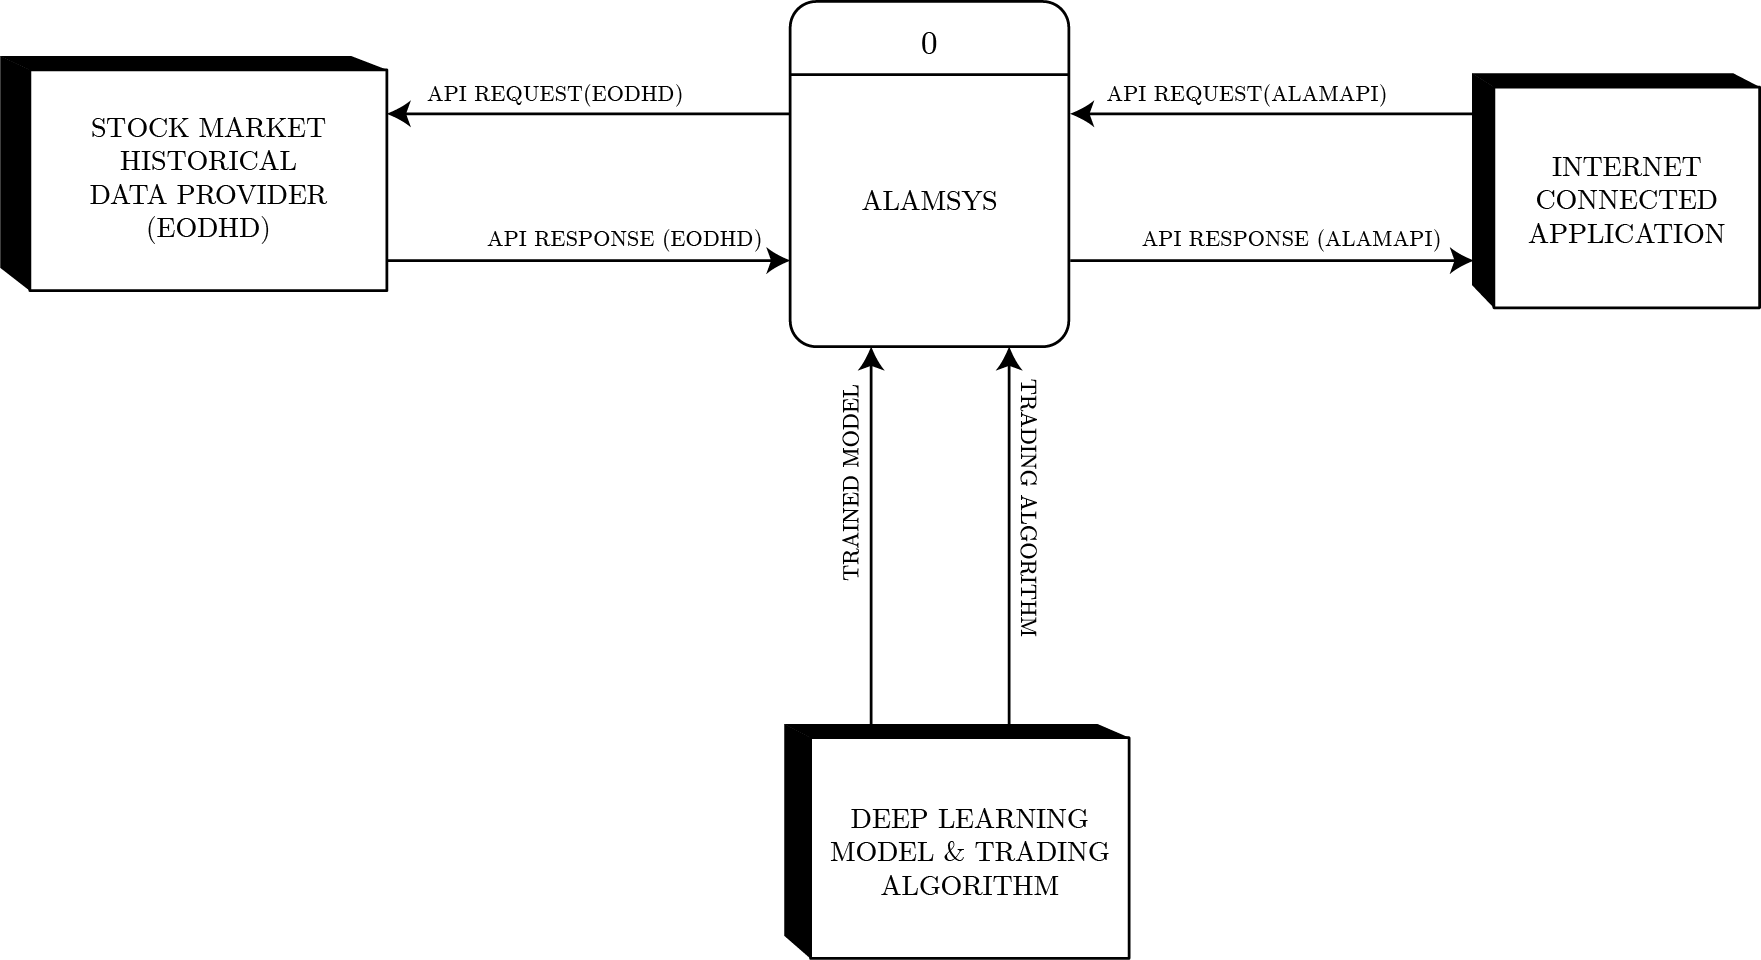
\includegraphics[width=0.80\textwidth]{./assets/Chapter_3/DFD/DFD_Context.png}
    \caption{Context Diagram of the alamSYS}
    \label{fig:context_dfd}
\end{figure}
\FloatBarrier
\vspace{0.5cm}
The diagram above depicts the root process (0), which is the alamSYS itself, 
and is linked to three external entities: 
(a) Stock Market Historical Data Provider, which was provided by EODHD;
(b) Deep Learning Model \& Trading Algorithm,these were developed alongside the 
alamSYS, specifically the DMD-LSTM Model and ALMACD, respectively; and 
(c) Internet Connected Applicatio, these are any type of applications with 
internet access. Other applications may include a web-based application, a 
smart home speaker, and so on.
\\

The data flow lines shown Figure \ref{fig:context_dfd} include the following:
(a) API Request(EODHD), this is the request sent to the EODHD API to collect the 
stock market historical data; 
(b) API Response(EODHD), this is the response received from the 
EODHD API, which contains the end of day stock market data; 
(c) API Request(alamAPI), this are the requests sent by any 
internet connected application to the alamSYS via the alamAPI; 
(d) API Response(alamAPI), this are the responses sent by the alamSYS to 
any internet connected application via the alamAPI;
(e) Trained Model, this is the trained model, referring to the DMD-LSTM, 
that was used to predict the price movement of the stocks in the Philippine 
Stock Market; and
(f) Trading Algorithm, this is the deployed trading algorithm, referring to the ALMACD,
that was used to determine the entry and exit signals of the stocks in the Philippine 
Stock Market.
\\

In connection, the following are the API requests that can be utilized:
(a) Home, this API endpoint returns a greeting message. Which should notify the 
user that they have connected to the alamAPI successfully;
(b) Stocks to Buy, these API endpoints return a json data of recommended stocks to 
buy based on the current market price, the predicted price uptrend, and the entry signal of the
trading algorithm in use;
(c) Stocks to Sell, these API endpoints return a json data of recommended stocks to 
sell based on the current market price, the predicted price downtrend, and the exit signal of the
trading algorithm in use;
(d) ML Model Info, these API endpoints return a json data of the Machine Learning Models 
used in the alamSYS, as well as their associated information; and 
(e) Stock Risks Profile, these API endpoints return a json data of stocks in the 
alamSYS as well as their risk values based on value at risk (\%), volatility (\%), 
and drawdown (\%).
\\

% DFD 0
\subsubsection{DFD of Diagram 0}
\label{subsubsec:dfd0}
To better understand how each data stream entering and exiting the root process is processed, 
it is essential to look inside the inner workings of the root process, which is illustrated in the DFD of Diagram 0, 
as shown in Figure \ref{fig:dfd0}.
\begin{figure}[ht]
    \centering
    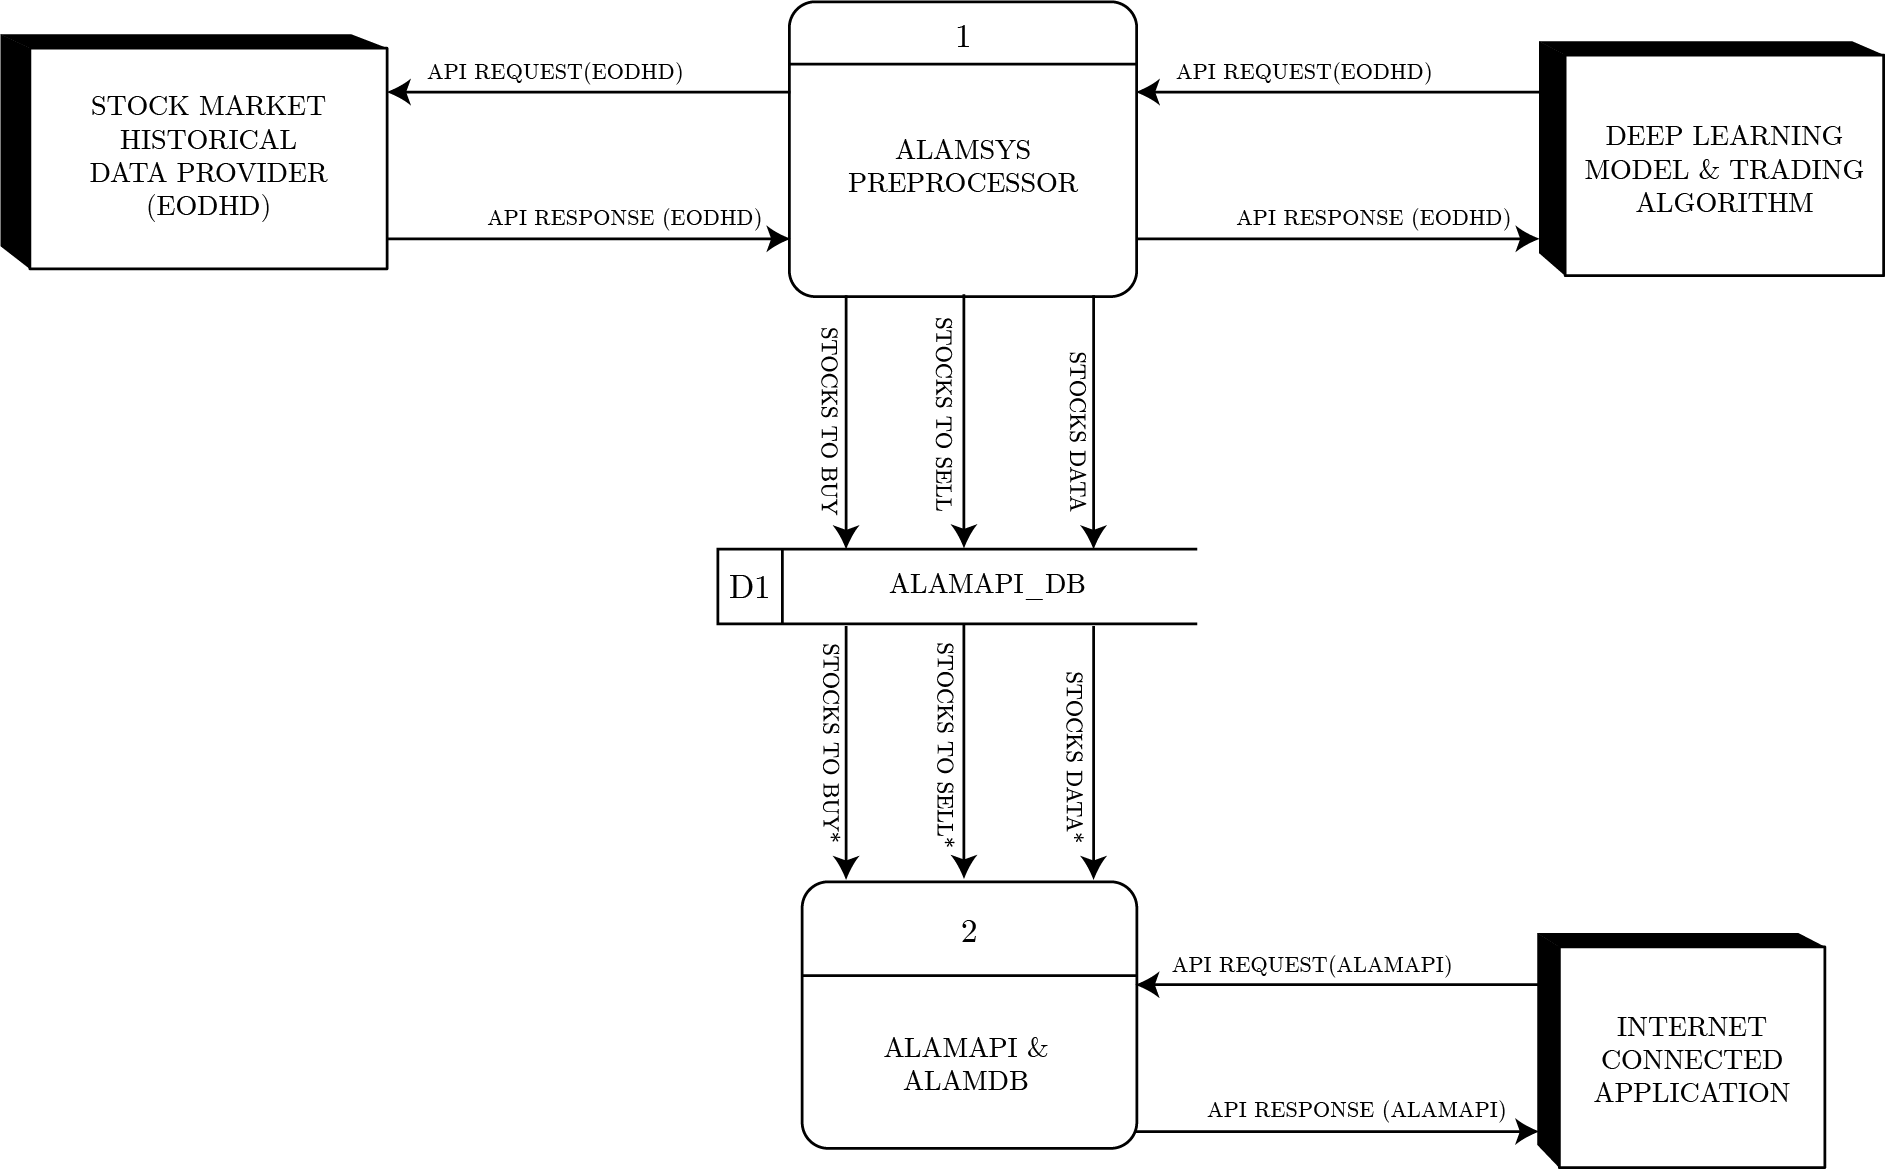
\includegraphics[width=0.80\textwidth]{./assets/Chapter_3/DFD/DFD_0.png}
    \caption{DFD of Diagram 0}
    \label{fig:dfd0}
\end{figure}
\FloatBarrier

From the figure above, the root process, has two main processes:
(a) alamSYS Preprocessor, which is the system’s stock market data processing unit, which deploys
the deep learning model (DMD-LSTM), and the trading algorithm (ALMACD) to predict the price movement of the
stocks in the Philippine Stock Market; and
(b) alamAPI \& alamDB, which is the system’s API and database unit, which is responsible for
processing the API requests and responses, as well as storing the data of 
the system, respectively.
\\

% DFD 1
\subsubsection{DFD of Diagram 1}
\label{subsubsec:dfd1}
To better understand the internal workings of the Process 1, 
it is useful to check the DFD of that process, which is illustrated in Figure \ref{fig:dfd1}
\begin{figure}[ht]
    \centering
    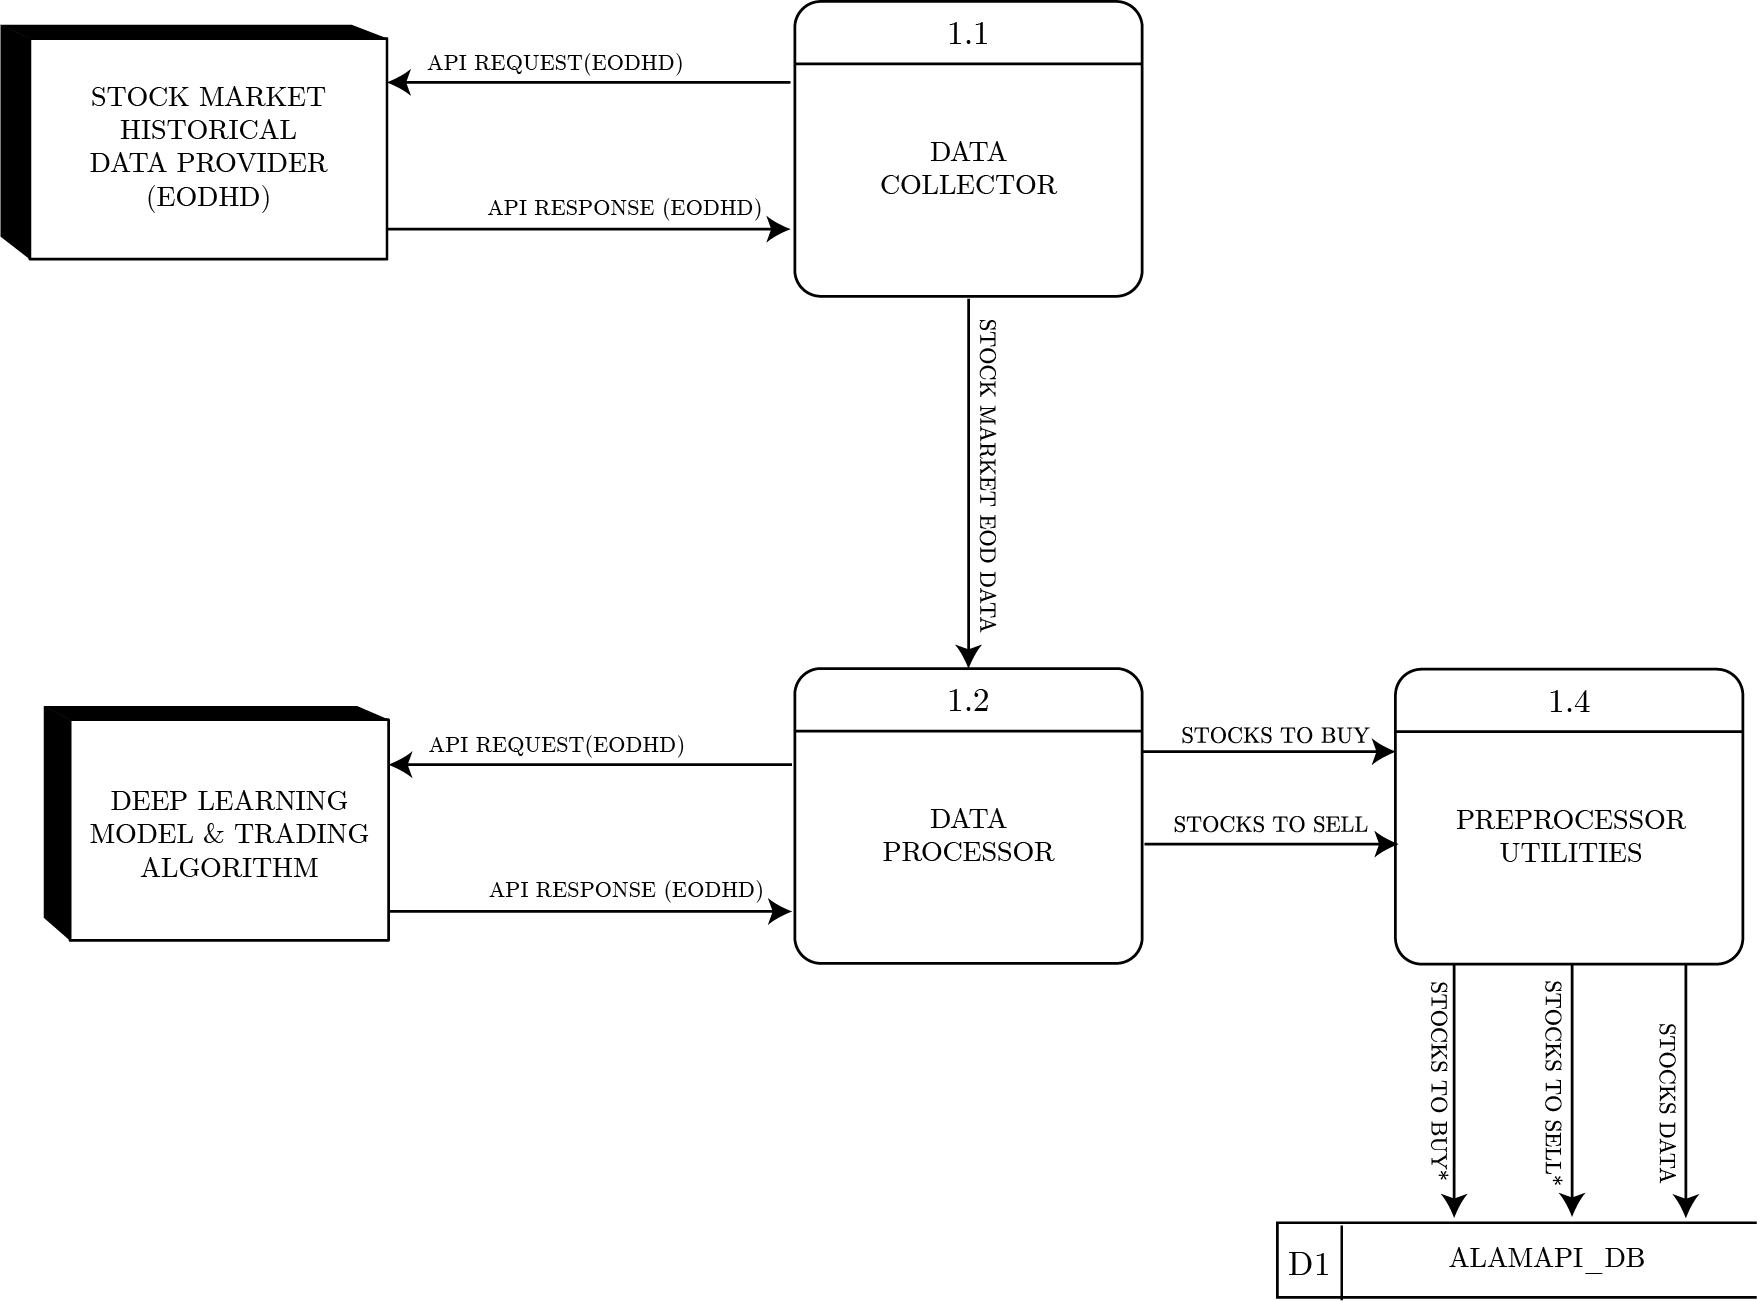
\includegraphics[width=0.80\textwidth]{./assets/Chapter_3/DFD/DFD_1.png}
    \caption{DFD of Diagram 1}
    \label{fig:dfd1}
\end{figure}
\FloatBarrier

From the figure shown above, it can be observed that Process 1 
is composed of three internal processes, which are as follows:
(a) Data Collector, which is the main process responsible 
for collecting the historical market data using EODHD End of Day Market Data API; 
(b) Data Processor, which is the main process responsible for processing the collected 
stock market data using the DMD-LSTM Model and the ALMACD Trading Algorithm; and
(c) Preprocessor Utilities, these are a set of tools that contains the 
utilities used by the data processor, such as the initialization of the database, database related actions, 
database models, stock symbols, and logs and alerts module.
\\

% DFD 1.2
\subsubsection{DFD of Diagram 1.2}
\label{subsubsec: dfd1.2}
This shows the processes inside the process 1.2, which is the data processor.
\begin{figure}[ht]
    \centering
    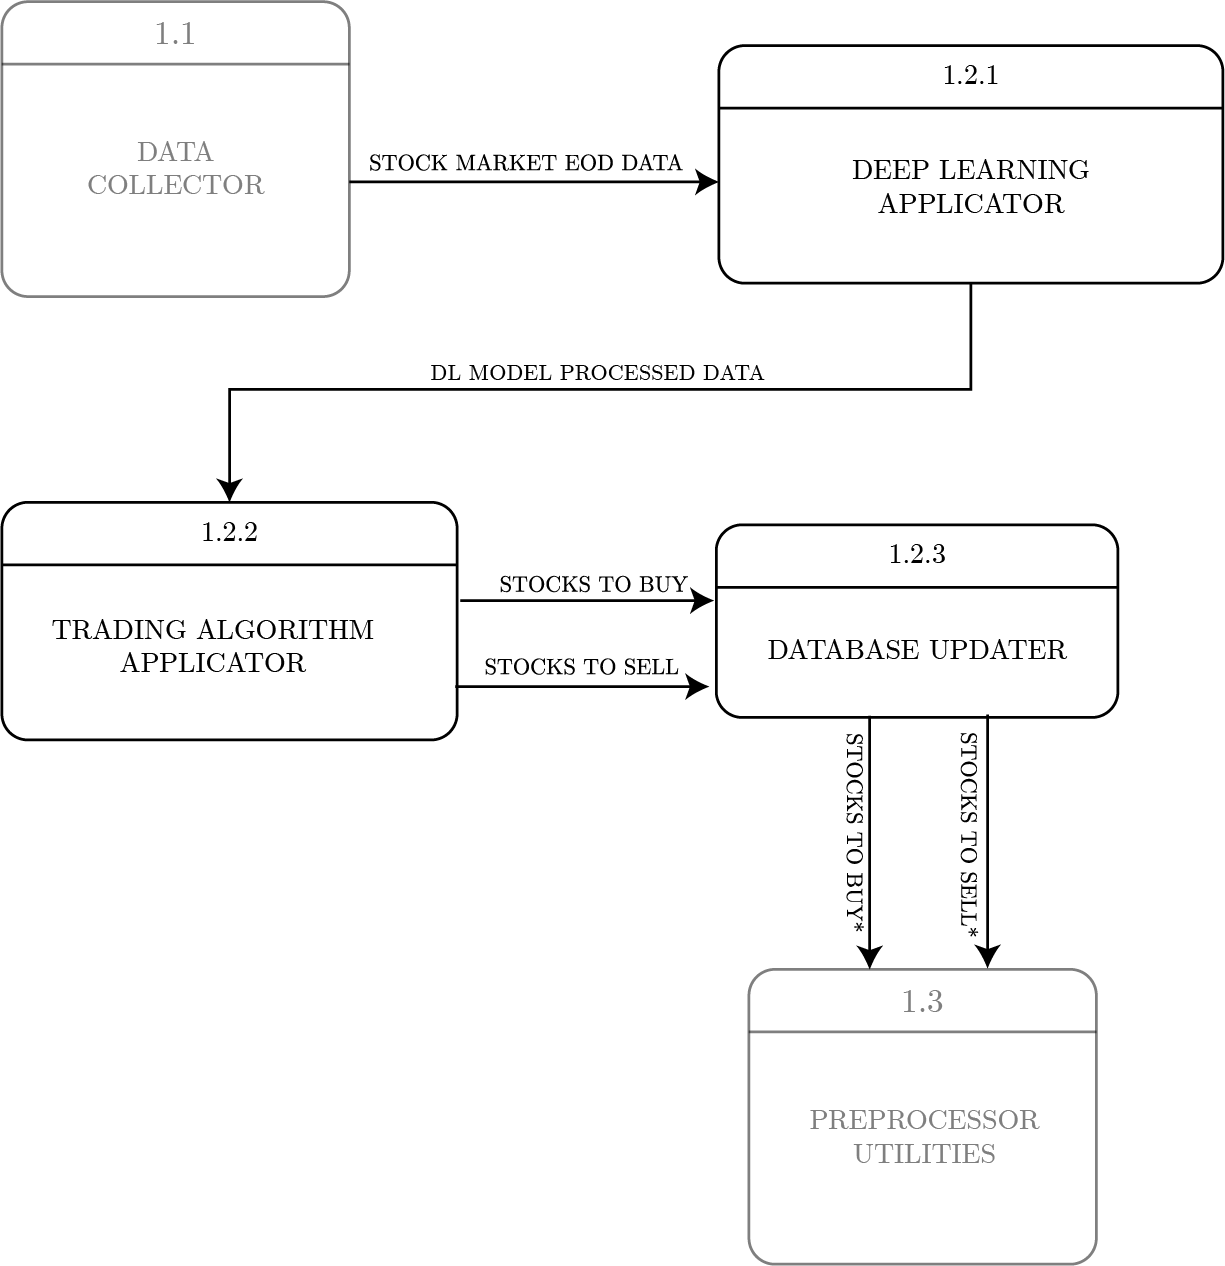
\includegraphics[width=0.80\textwidth]{./assets/Chapter_3/DFD/DFD_1.2.png}
    \caption{DFD of Diagram 1.2}
    \label{fig:dfd1.2}
\end{figure}
\FloatBarrier

The data processor is further composed of three processes, which are as follows:
(a) Deep Learning Applicator, this subprocess applies the DMD-LSTM model to 
the collected stock market end-of-day (eod) data; 
(b) Trading Algorithm Applicator, the eod data alongside the list of predicted stock prices
composes the "DL Model Processed Data", which is sent to this subprocess. 
This subprocess applies the ALMACD to better determine the entry (buy or hold), 
and exit (sell) signals for each stocks; and 
(c) Database Updater, a subprocess responsible for updating the contents of the database, 
based on the data processed by the Deep Learning Applicator and Trading Algorithm Applicator.
\\

% DFD 2
\subsubsection{DFD of Diagram 2}
\label{subsubsec:dfd2}
Figure \ref{fig:dfd2} shows the inner processes of the Process 2 (alamAPI \& alamDB).
\begin{figure}[ht]
    \centering
    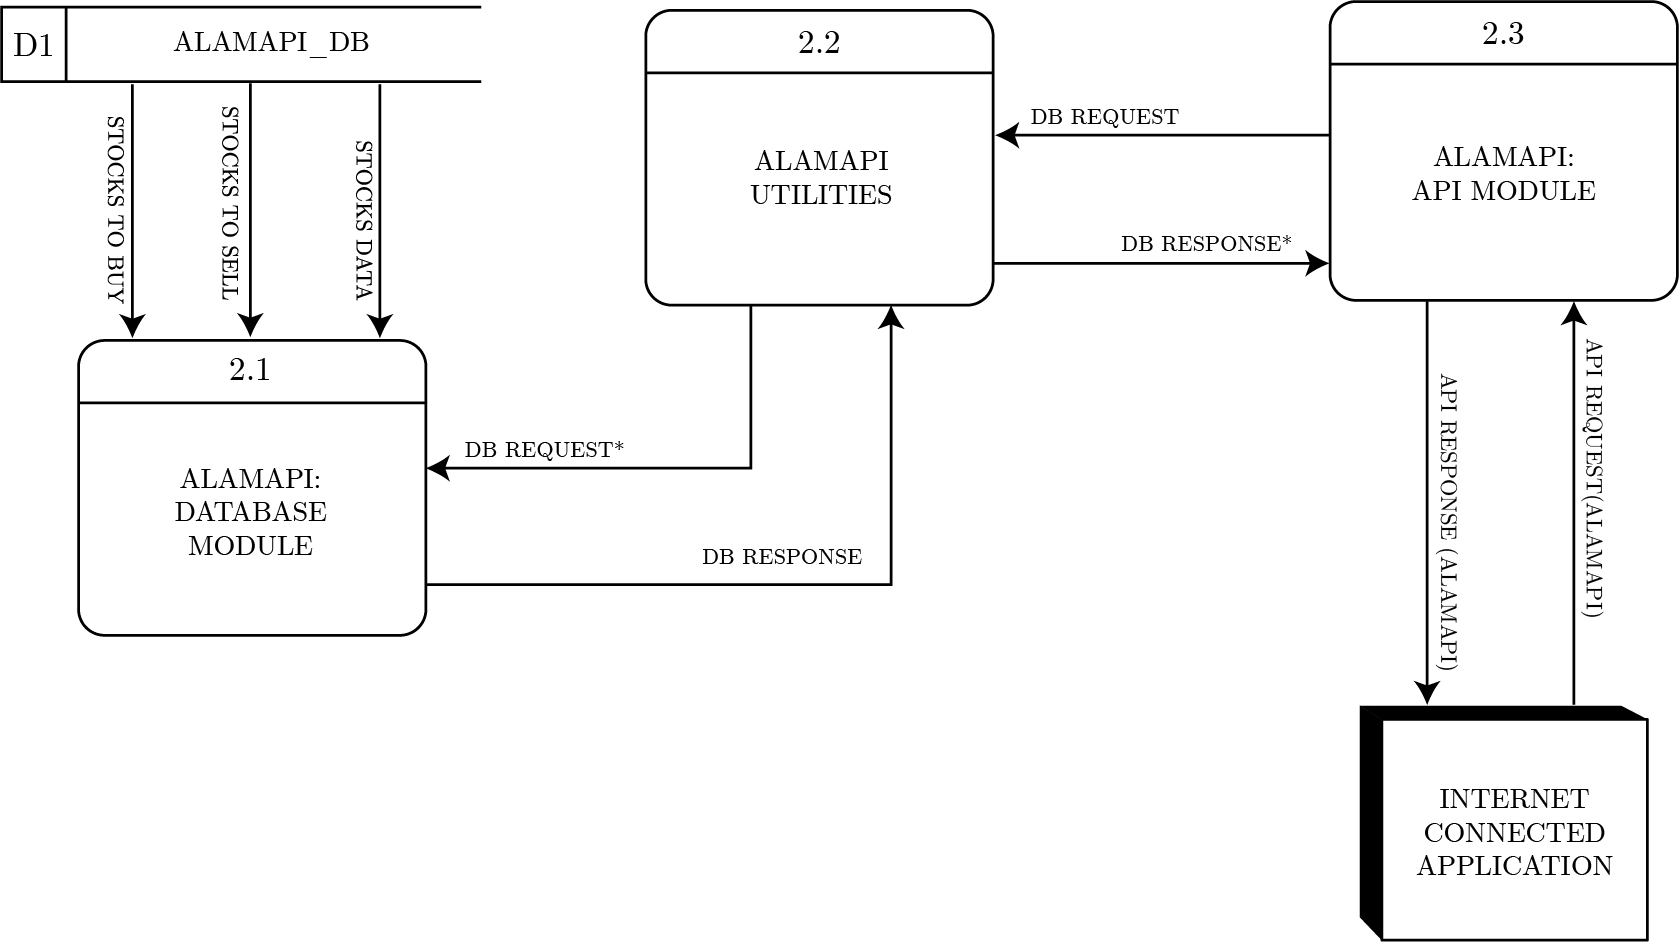
\includegraphics[width=0.80\textwidth]{./assets/Chapter_3/DFD/DFD_2.png}
    \caption{DFD 2: Data-Flow Diagram for the alamSYS}
    \label{fig:dfd2}
\end{figure}
\FloatBarrier


The figure above shows three internal processes of the Process 2, namely:
(a) alamDB, this process, processes the database request sent by the alamAPI as requested by the
Internet Connected Application through the utilization of alamAPI utilities. It also sends the database
response to the alamAPI via the same utilities module; 
(b) alamAPI Utilities, this process serves as a mediator of database request and responses
between the alamDB and alamAPI; and 
(c) alamAPI, this process contains all the API endpoints for the alamAPI, which is responsible
for processing the requests and API responses from and to the connected users.
\\